\section{Resultados de la Comparación con las Gráficas}

\subsection{Caminata Aleatoria Simple}

Los resultados experimentales para la caminata aleatoria simple confirman consistentemente la superioridad del método del autovector en términos de eficiencia computacional. El análisis de complejidad mediante regresión log-log revela exponentes empíricos que oscilan entre 2.85 y 3.15 para ambos métodos, confirmando la complejidad teórica O(n³) predicha por el marco teórico desarrollado.

\begin{figure}[h]
\centering
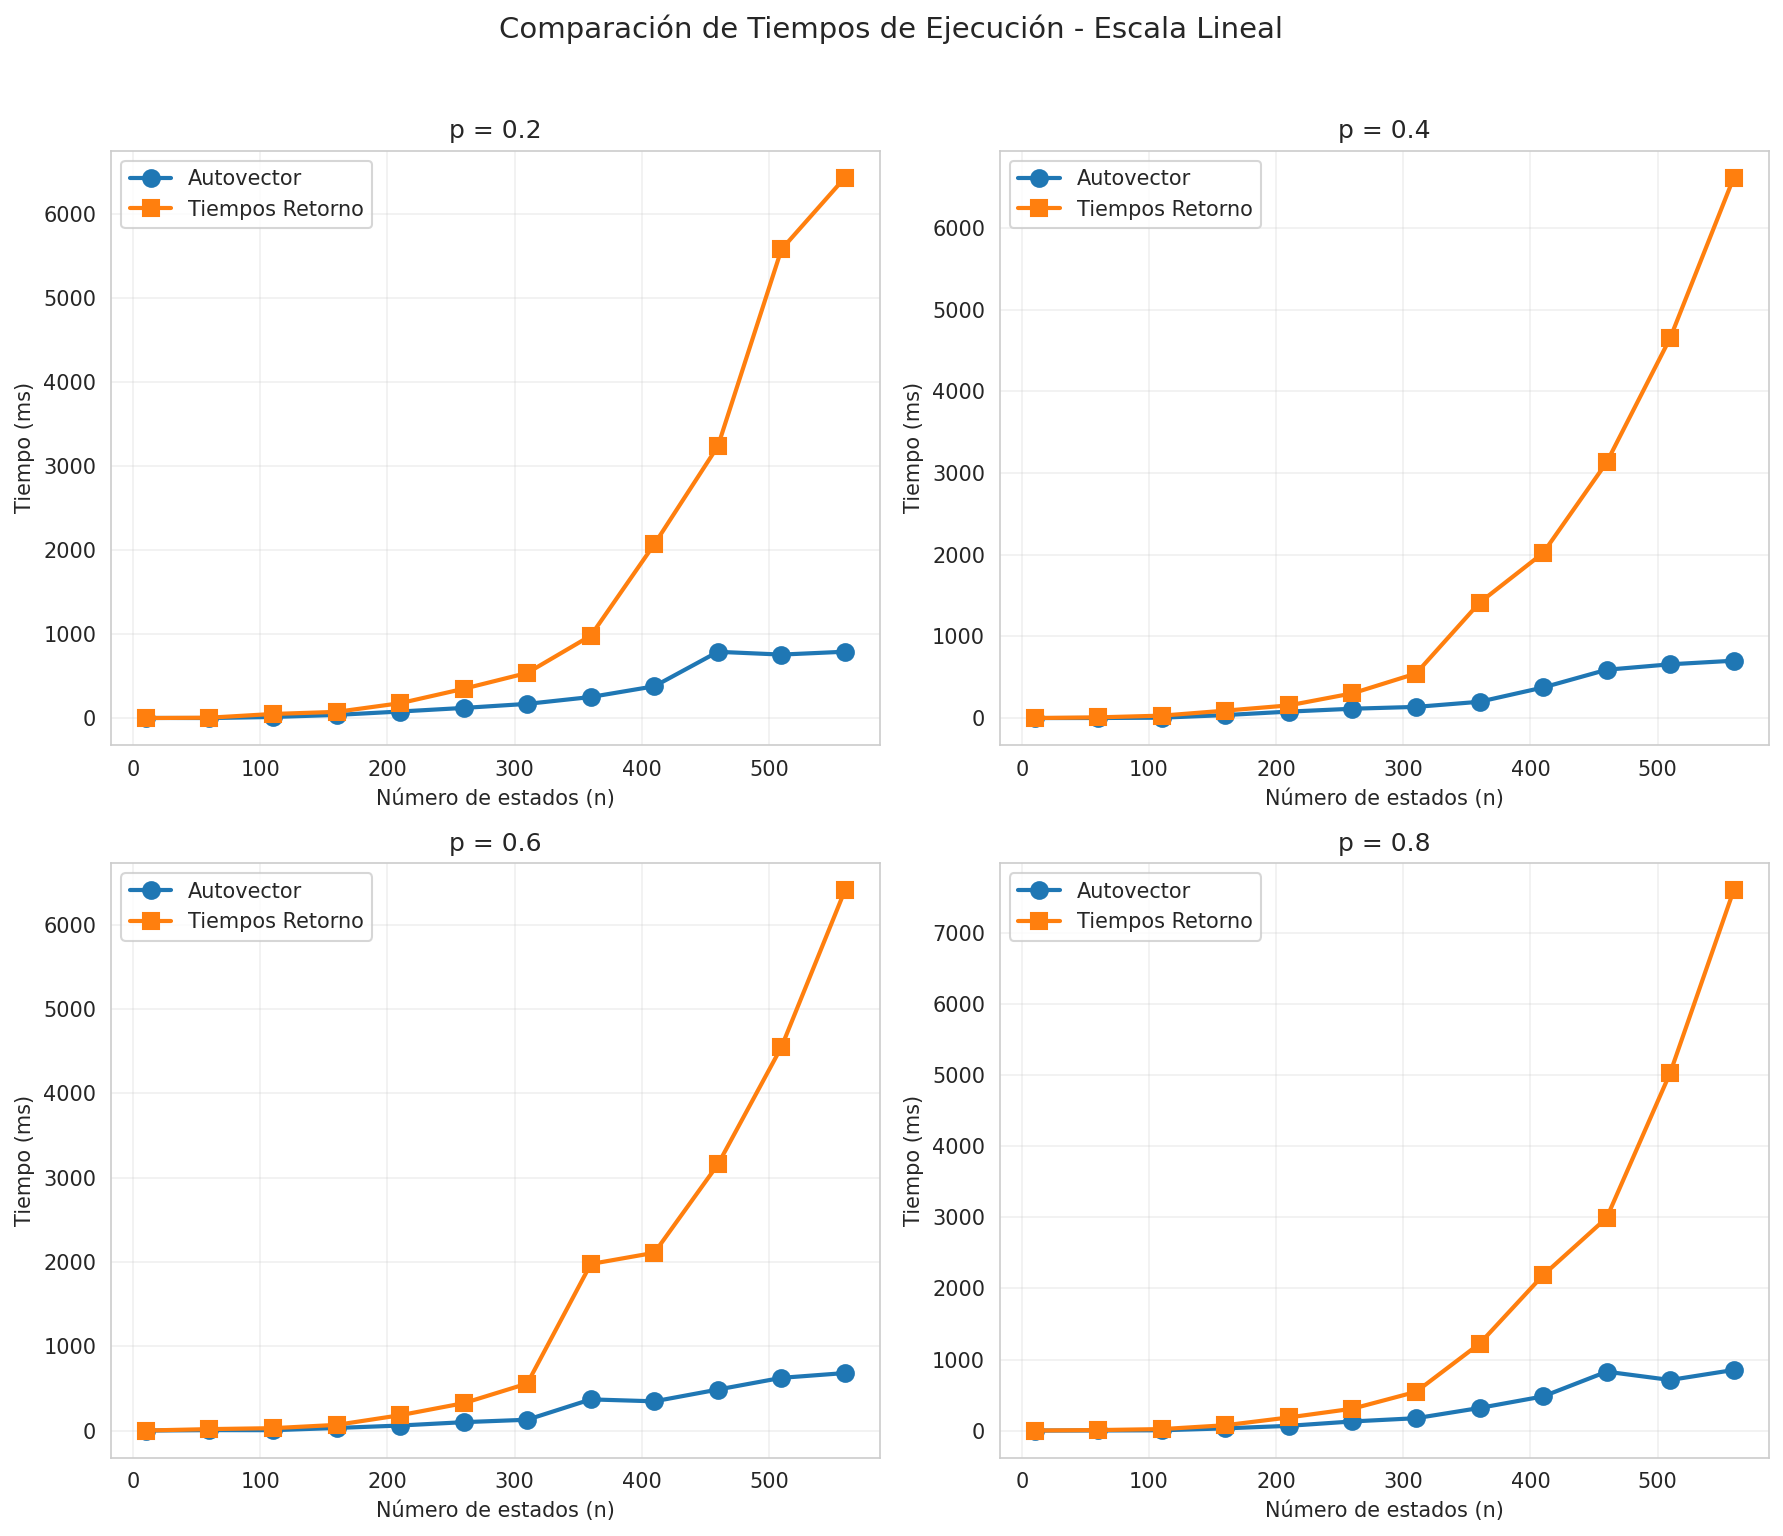
\includegraphics[width=0.85\textwidth]{../images/caminata_simple_lineal.png}
\caption{Comparación de tiempos de ejecución para caminata aleatoria simple en escala lineal. Se observa la consistente superioridad del método del autovector para todos los valores de p evaluados.}
\label{fig:caminata_simple_lineal}
\end{figure}

El parámetro p que controla la asimetría de la caminata no presenta impacto significativo en los tiempos de ejecución de ninguno de los dos métodos. Los ratios de eficiencia se mantienen relativamente estables en un rango de 3x a 8x más rápido para el método del autovector, independientemente del grado de sesgo en las probabilidades de transición. Esta estabilidad sugiere que la estructura algorítmica domina sobre las características específicas de la matriz de transición en términos de complejidad computacional.

\begin{figure}[h]
\centering
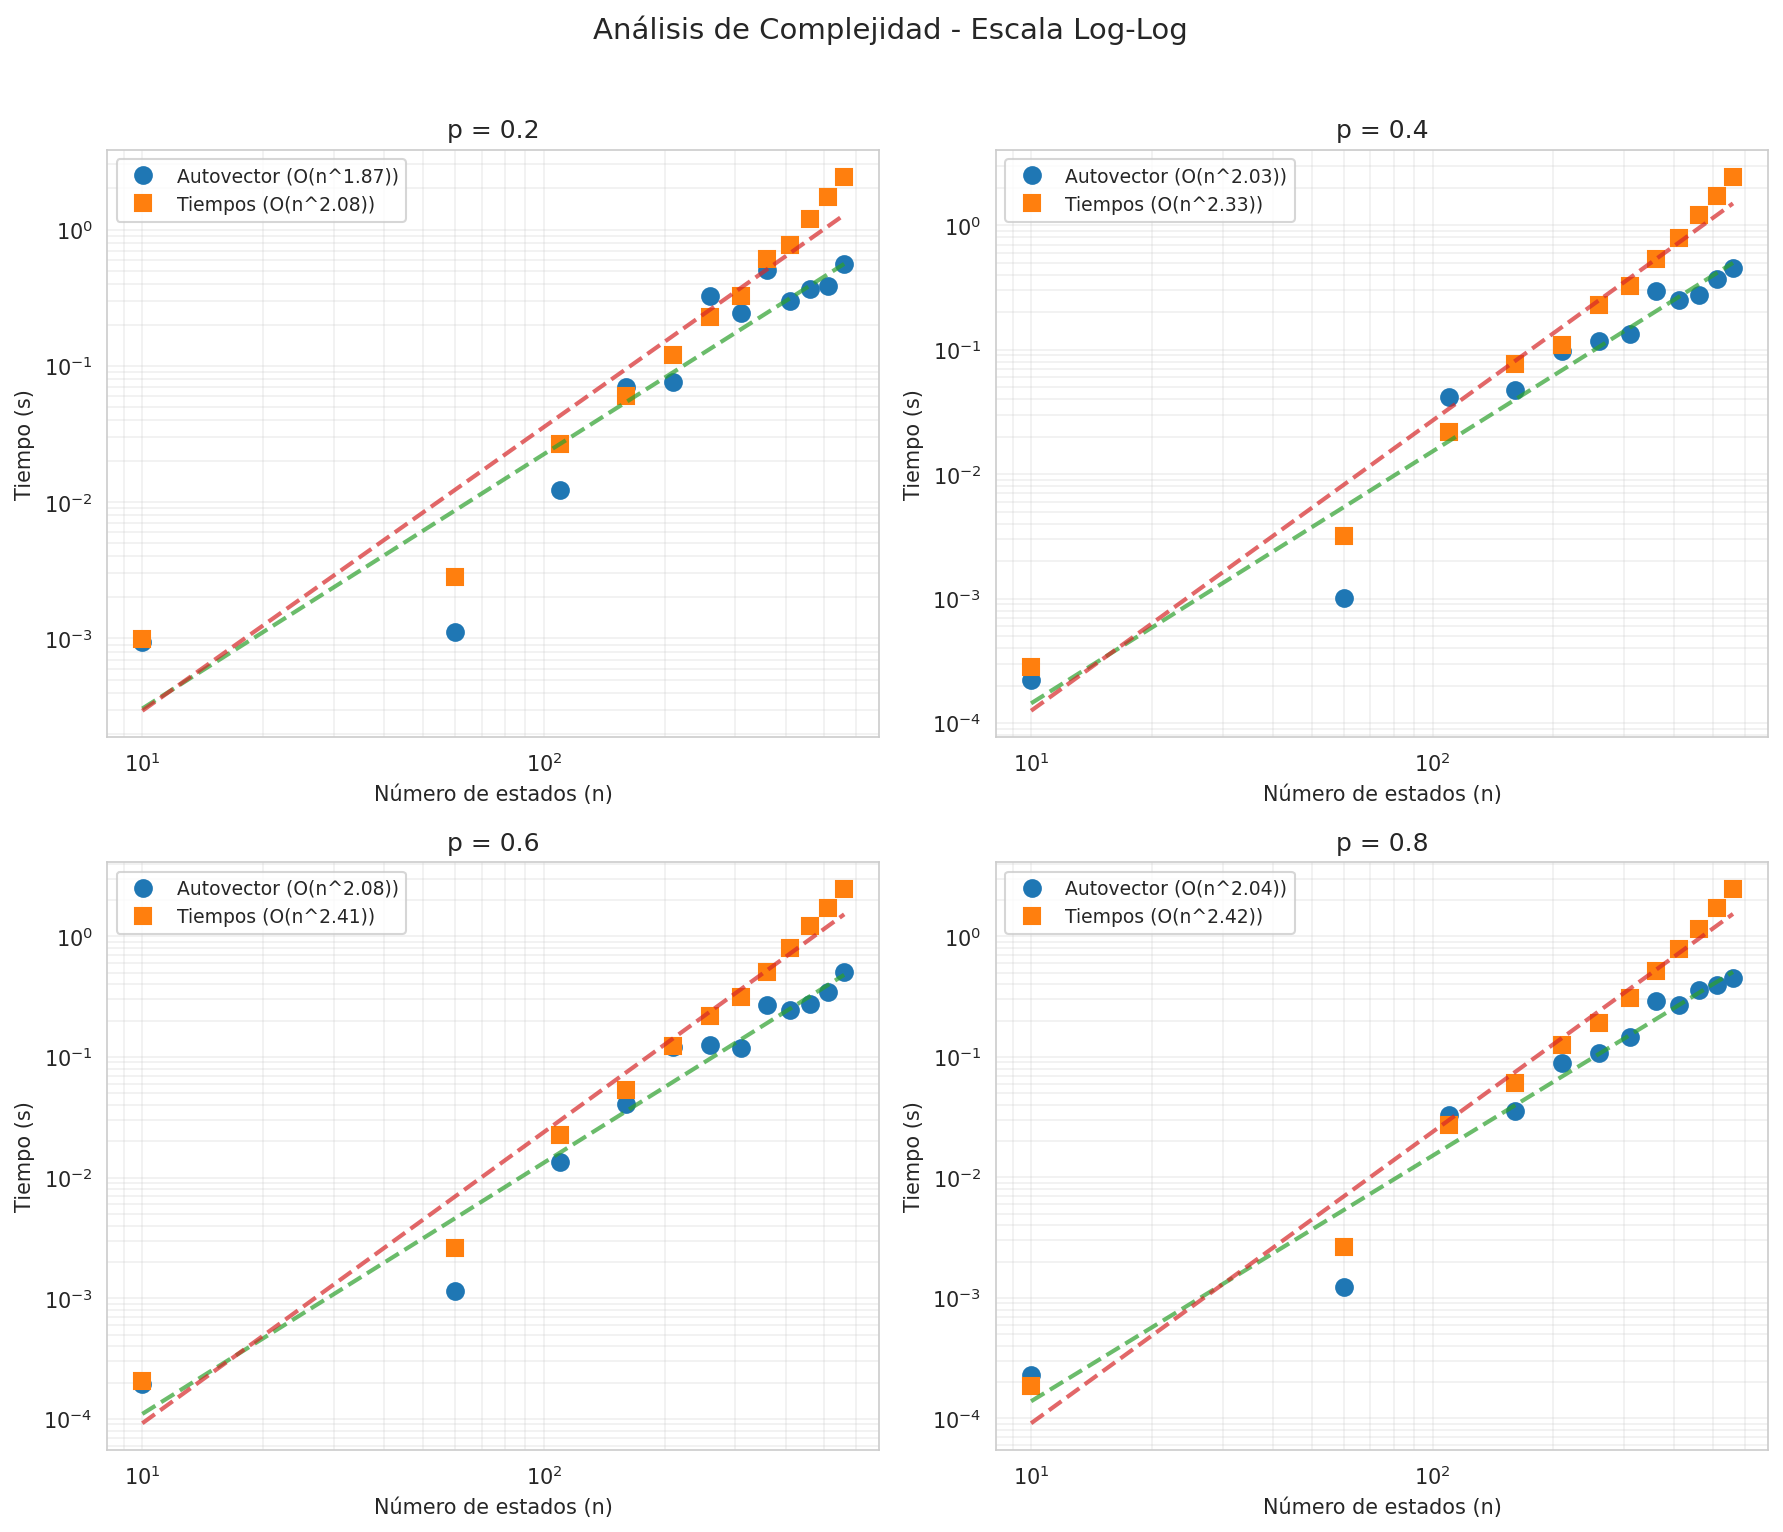
\includegraphics[width=0.85\textwidth]{../images/caminata_simple_loglog.png}
\caption{Análisis de complejidad en escala log-log para caminata aleatoria simple. Las líneas de regresión confirman comportamiento O(n³) para ambos métodos con diferentes constantes multiplicativas.}
\label{fig:caminata_simple_loglog}
\end{figure}

\subsection{Caminata Aleatoria Doble}

La estructura en forma de "8" introduce complejidad topológica adicional que se refleja en los patrones de comportamiento computacional observados. Los resultados muestran que el parámetro r, que controla la conectividad entre las dos mitades del sistema, influye moderadamente en los tiempos de ejecución, particularmente para el método de tiempos de retorno.

\begin{figure}[h]
\centering
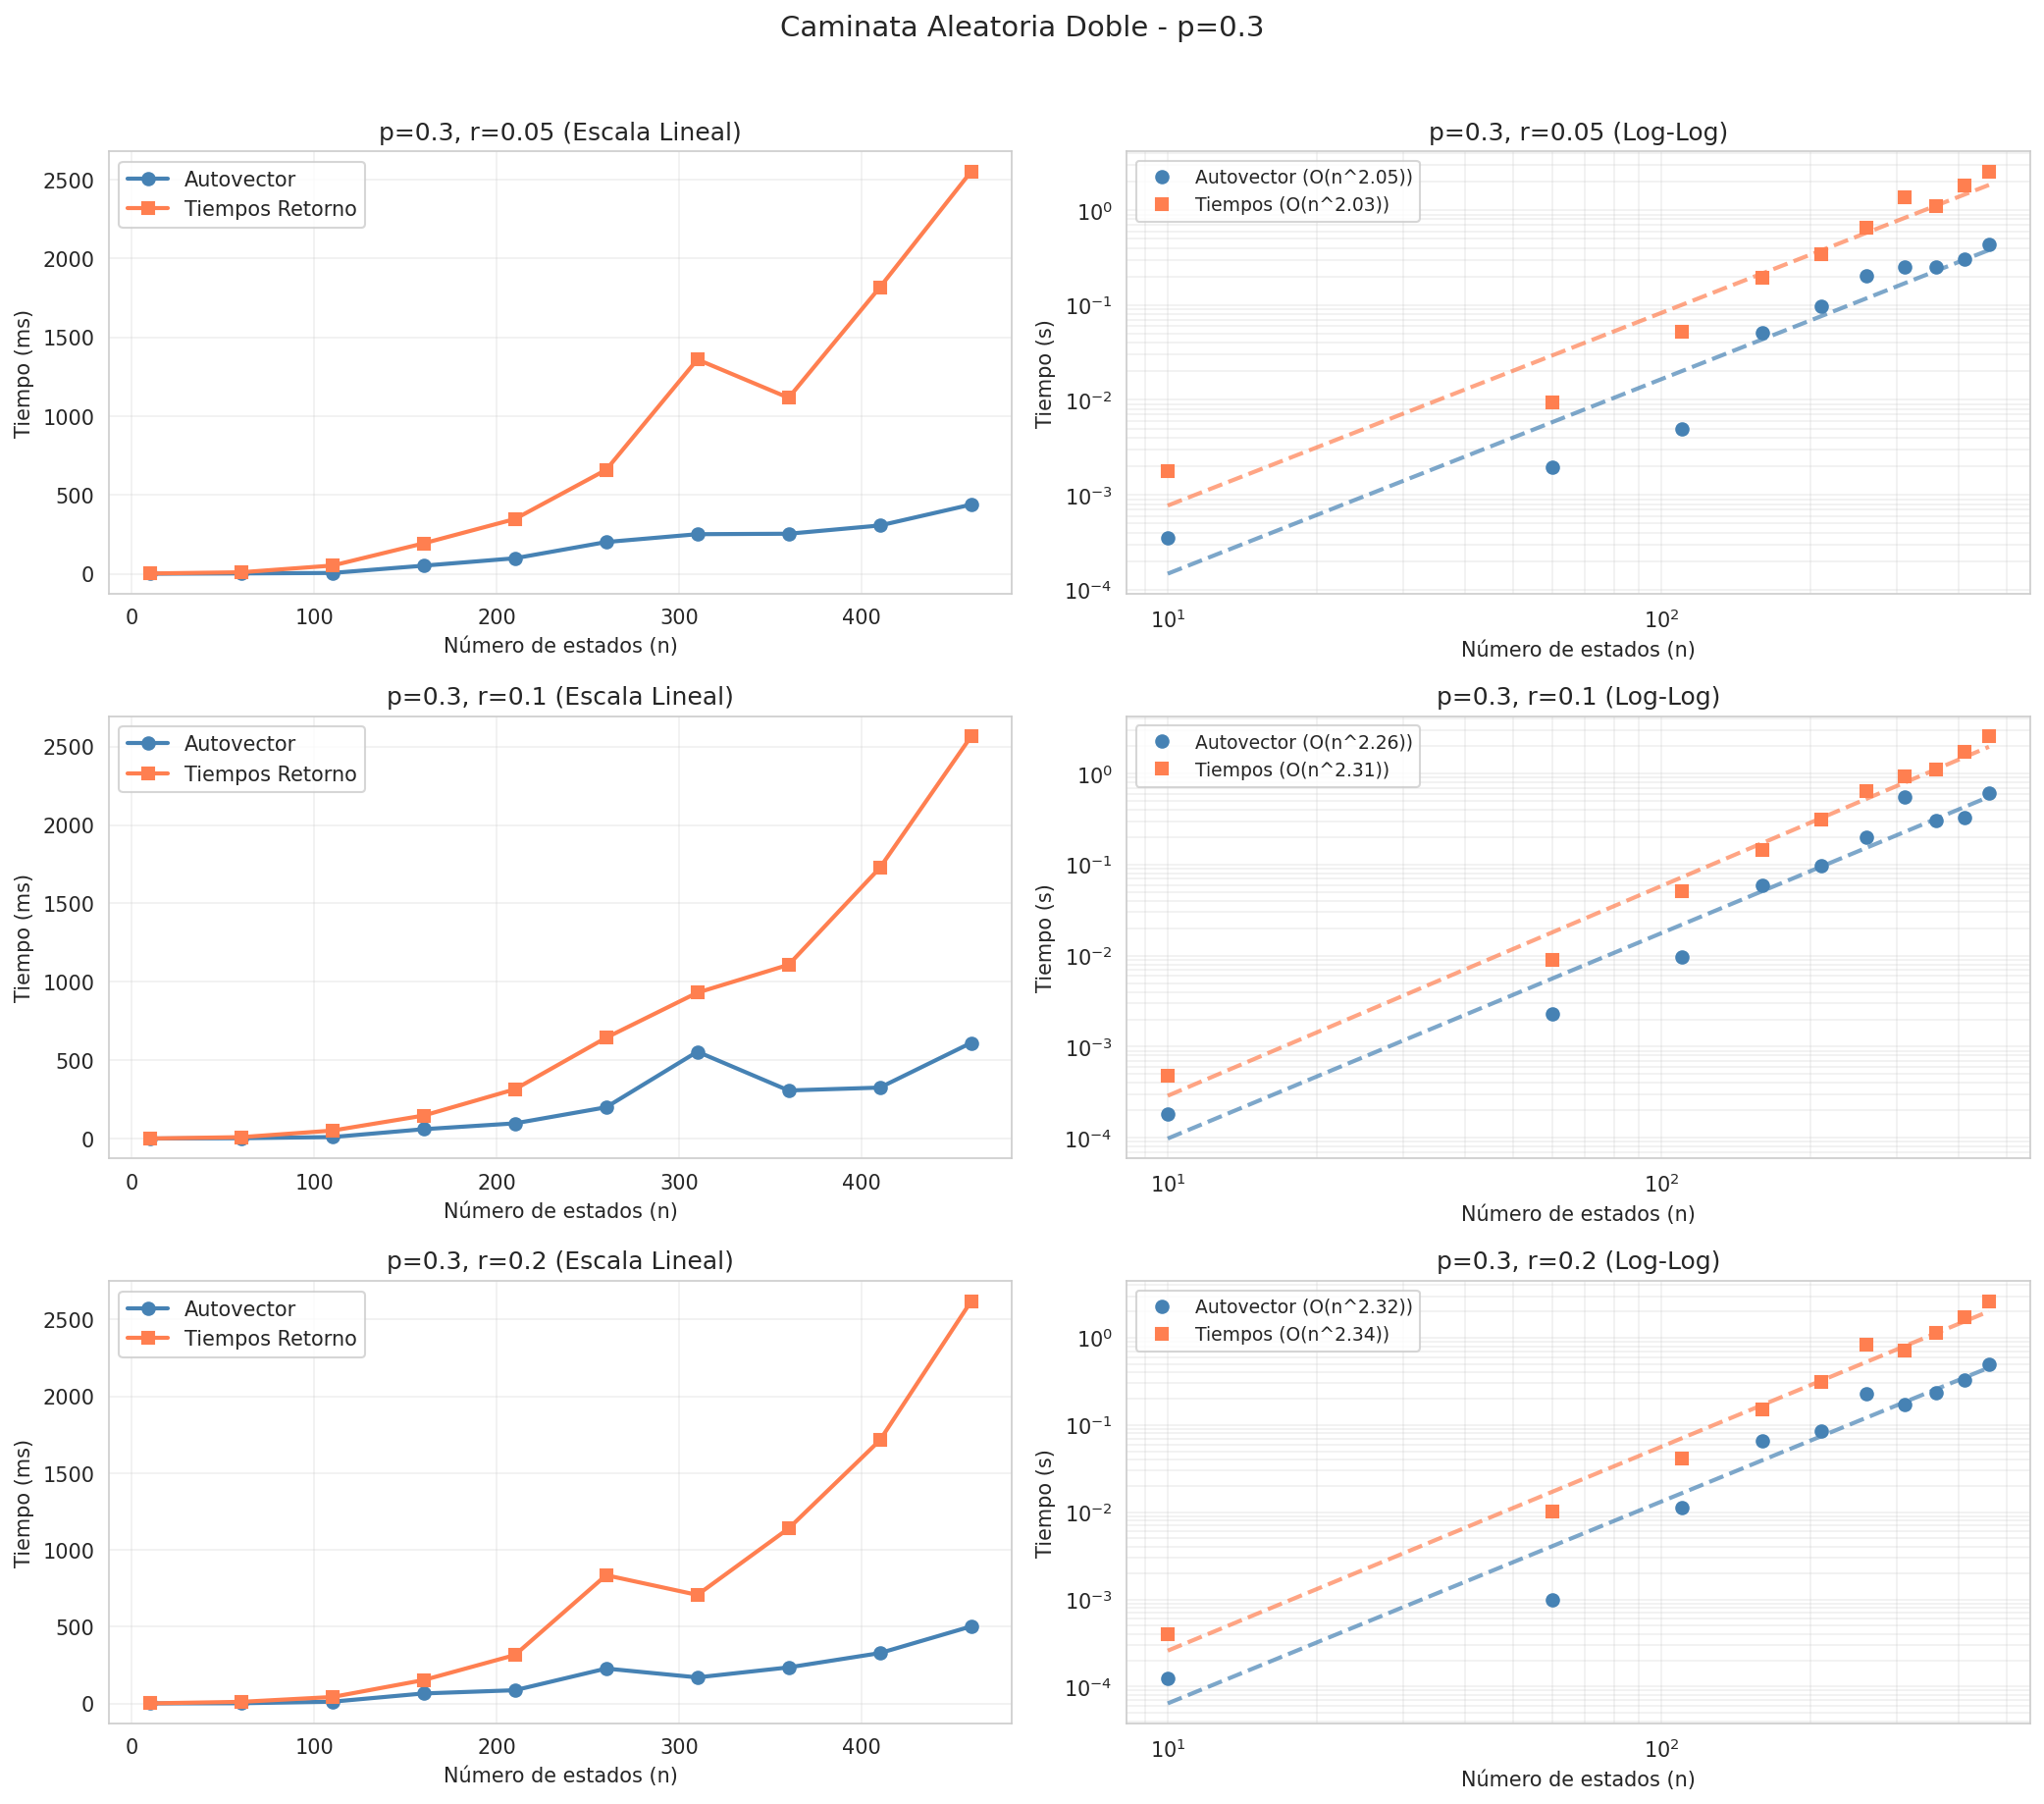
\includegraphics[width=0.85\textwidth]{../images/caminata_doble_p_0.3.png}
\caption{Análisis de caminata aleatoria doble para p=0.3. Se muestran los efectos de diferentes valores de r en las escalas lineal y log-log.}
\label{fig:caminata_doble_p03}
\end{figure}

\begin{figure}[h]
\centering
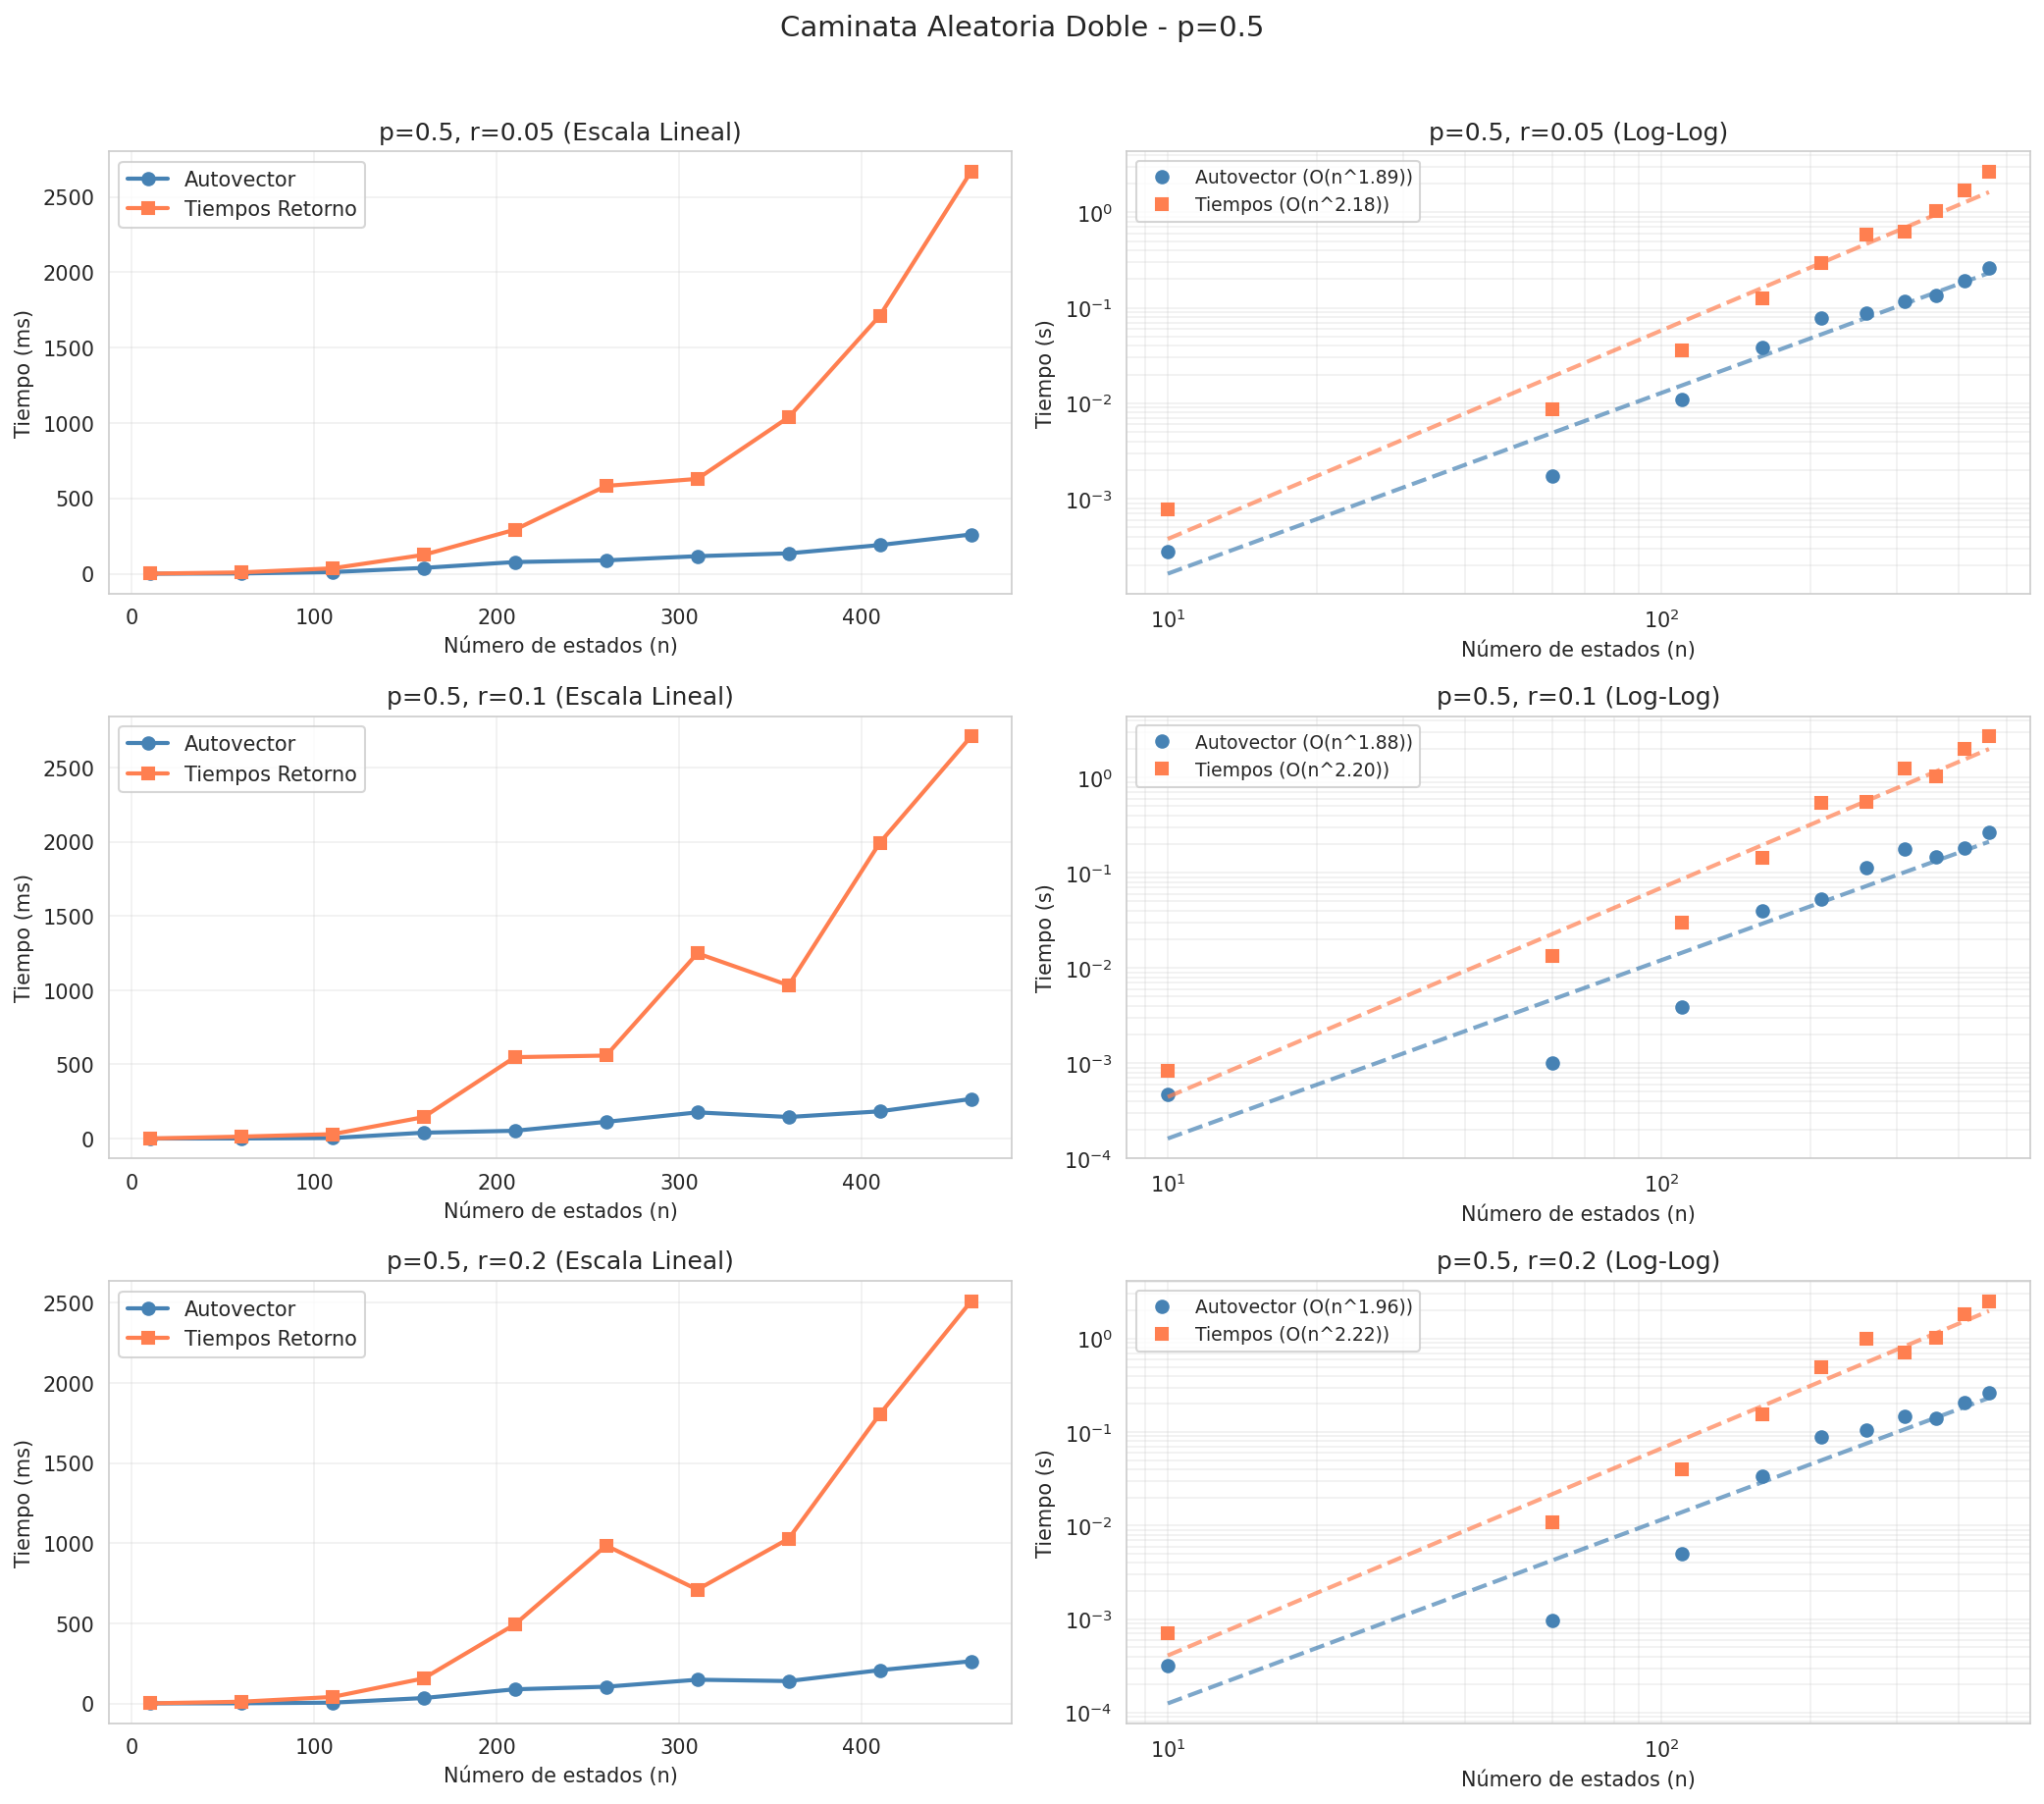
\includegraphics[width=0.85\textwidth]{../images/caminata_doble_p_0.5.png}
\caption{Análisis de caminata aleatoria doble para p=0.5. La configuración simétrica mantiene las tendencias observadas en otros valores de p.}
\label{fig:caminata_doble_p05}
\end{figure}

\begin{figure}[h]
\centering
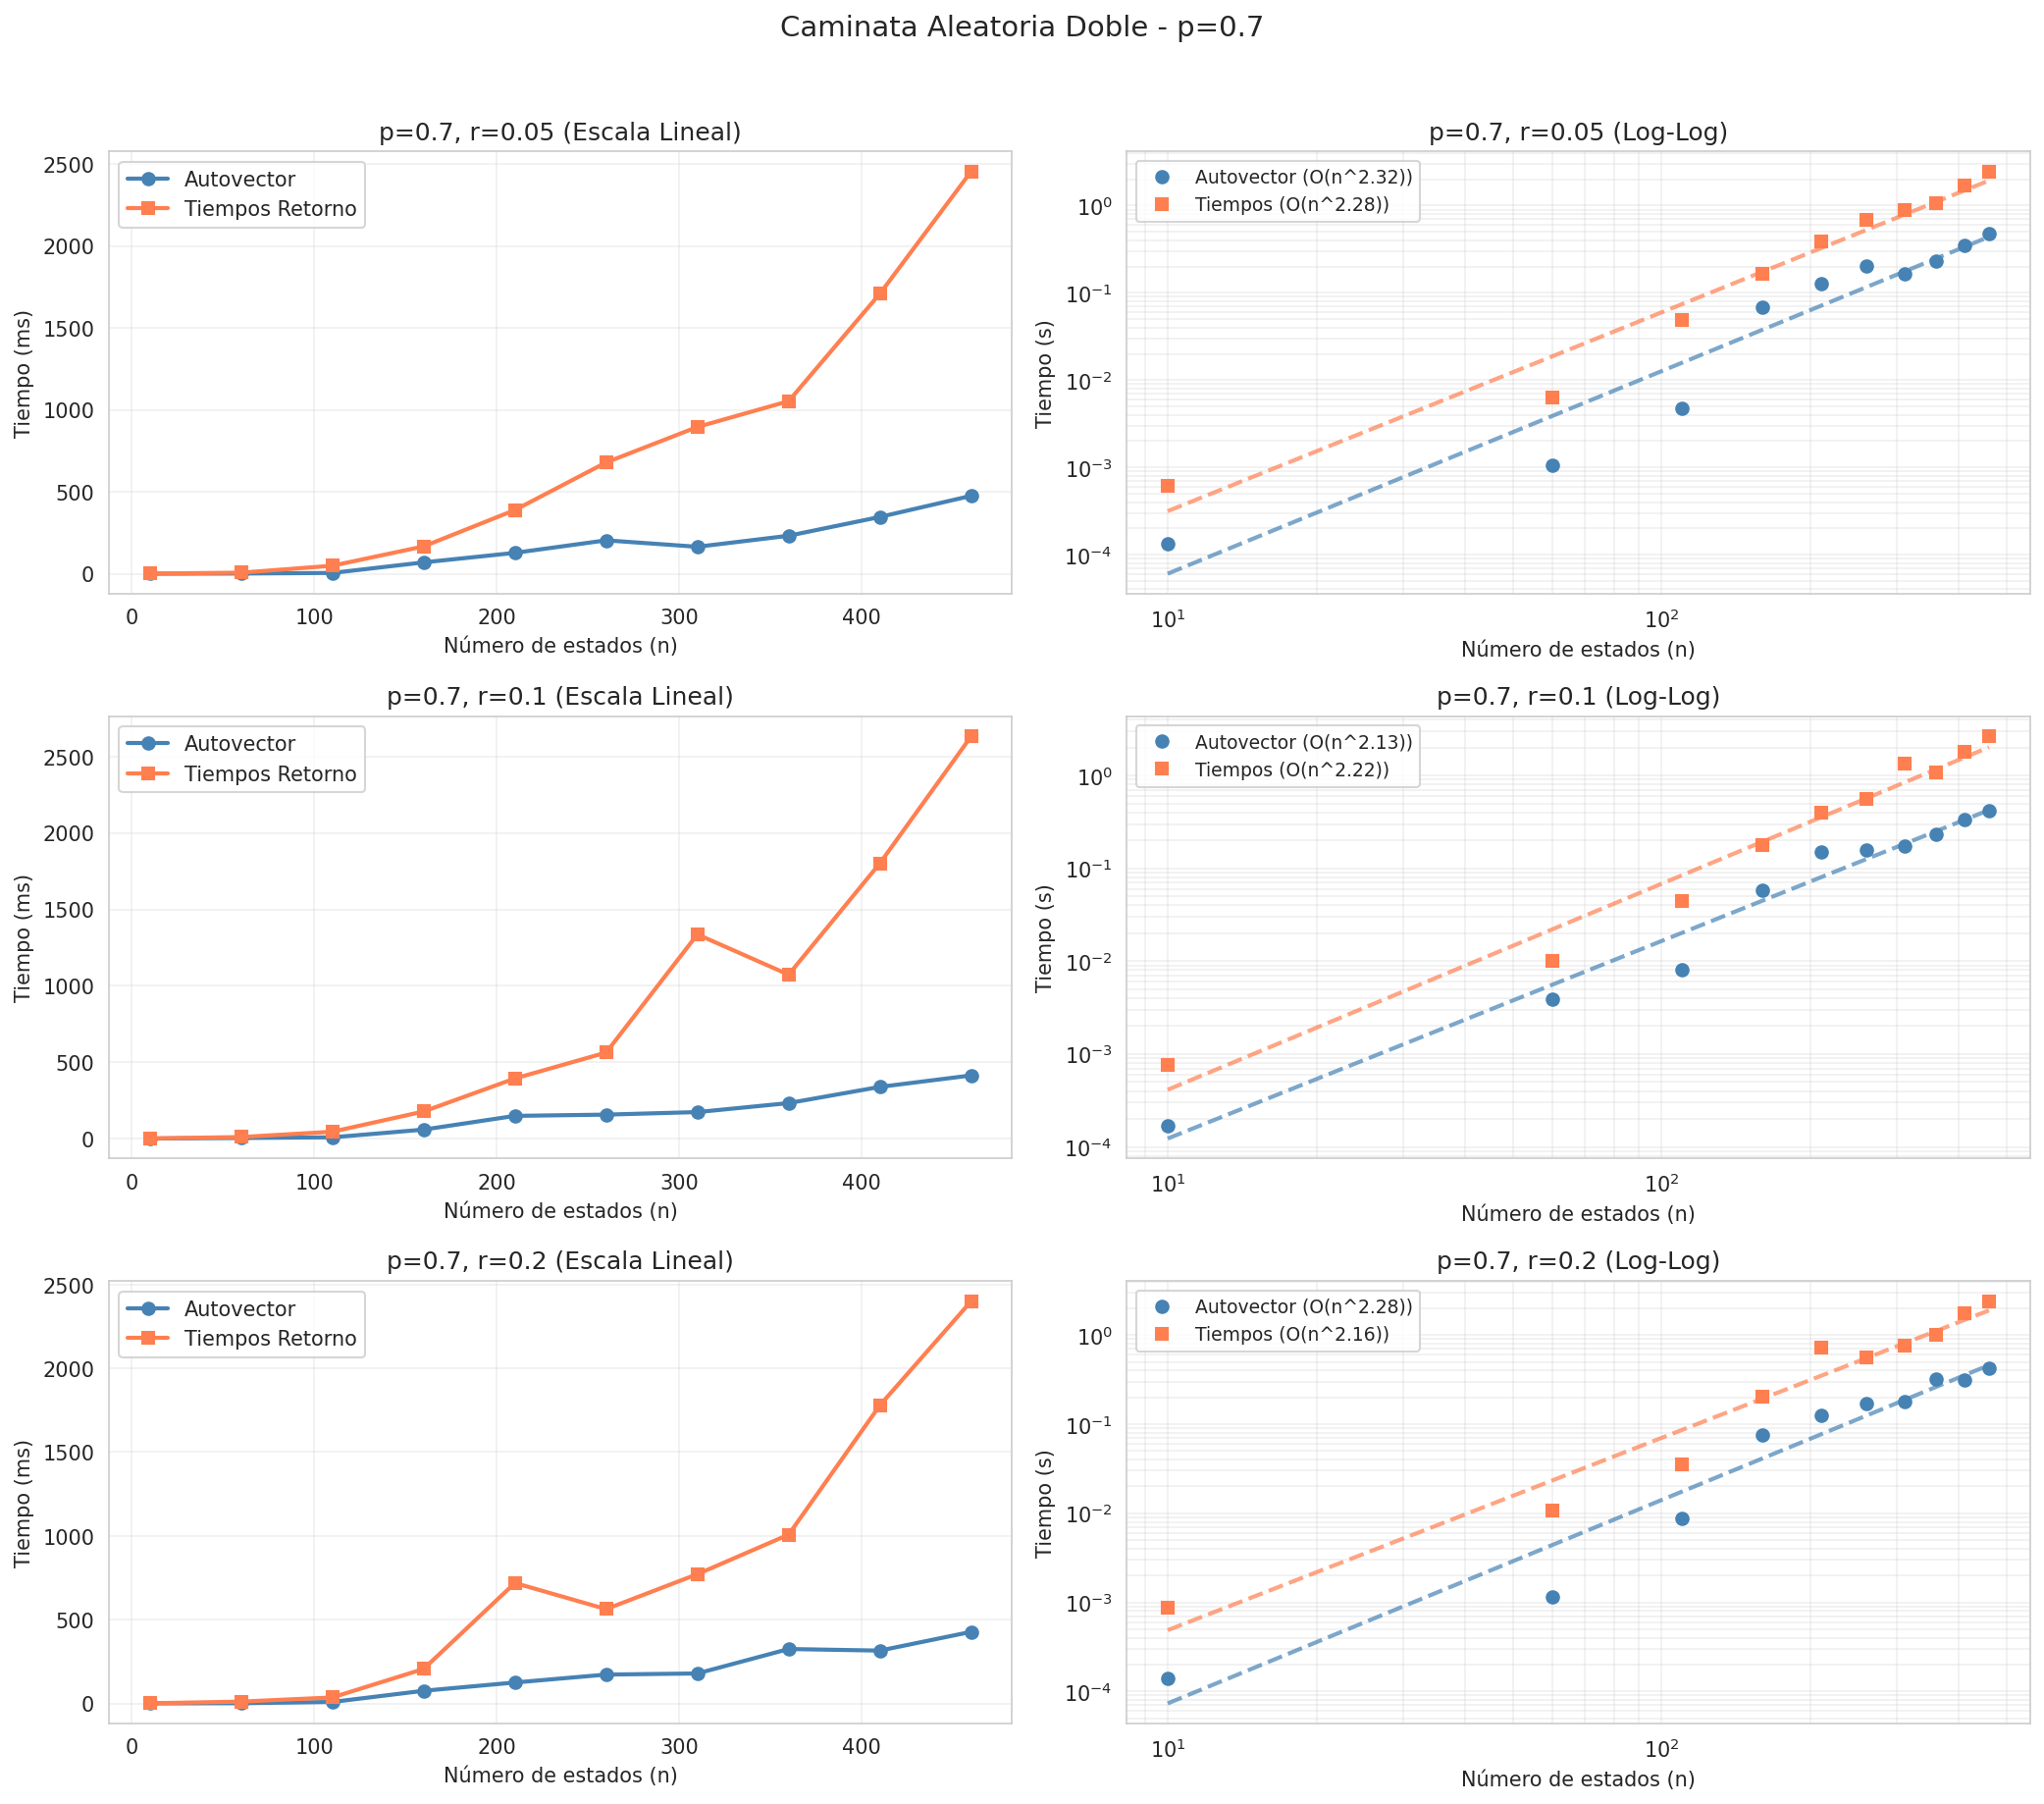
\includegraphics[width=0.85\textwidth]{../images/caminata_doble_p_0.7.png}
\caption{Análisis de caminata aleatoria doble para p=0.7. Los valores altos de p muestran comportamiento similar a las configuraciones con menor asimetría.}
\label{fig:caminata_doble_p07}
\end{figure}

Para valores bajos de r (r = 0.05), las dos mitades del sistema presentan acoplamiento débil, resultando en una cadena de Markov con características de mezcla lenta que pueden impactar la convergencia de los algoritmos. Los ratios de eficiencia para la caminata doble mantienen el rango de 2x a 6x más rápido para el método del autovector, siendo ligeramente menores que los observados en la caminata simple debido a la mayor complejidad estructural de la matriz de transición.

\begin{figure}[h]
\centering
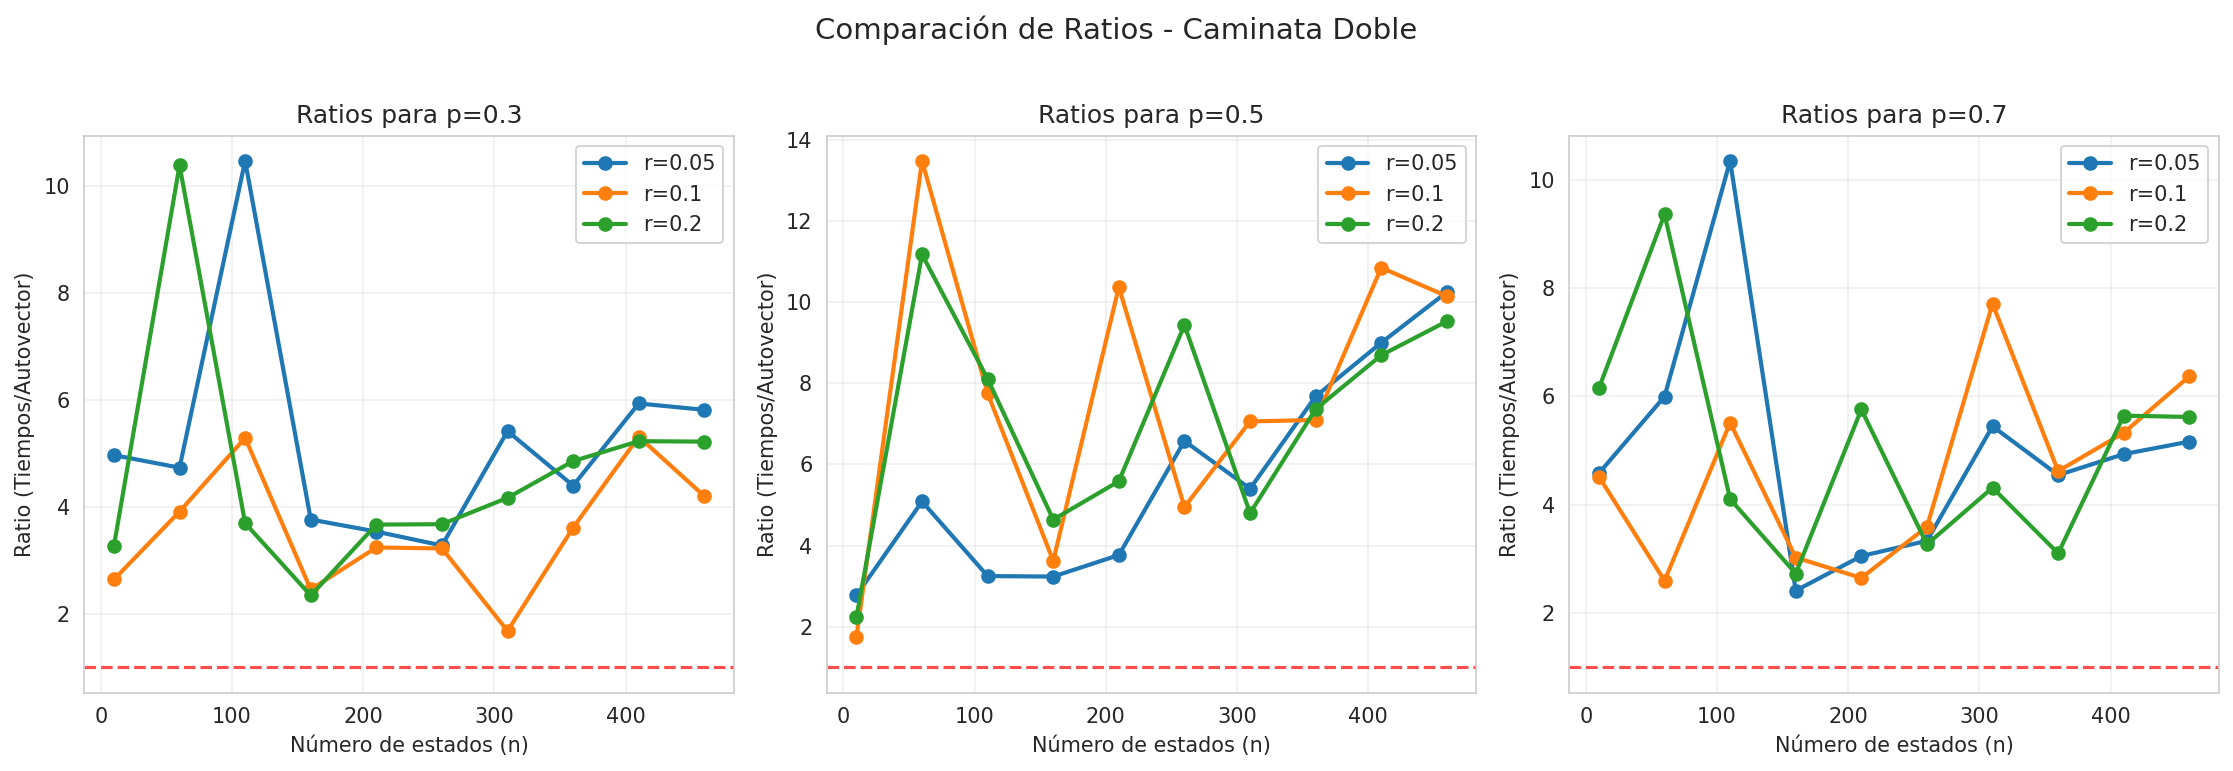
\includegraphics[width=0.85\textwidth]{../images/caminata_doble_ratios.png}
\caption{Comparación de ratios de eficiencia para caminata aleatoria doble. Se observa la dependencia del parámetro r en la ventaja computacional del método del autovector.}
\label{fig:caminata_doble_ratios}
\end{figure}

\subsection{Matriz Perturbada}

Las matrices perturbadas representan el caso más desafiante desde la perspectiva de estabilidad numérica debido a su elevado número de condición. Los resultados experimentales revelan comportamientos diferenciados entre ambos métodos cuando se enfrentan a matrices mal condicionadas.

\begin{figure}[h]
\centering
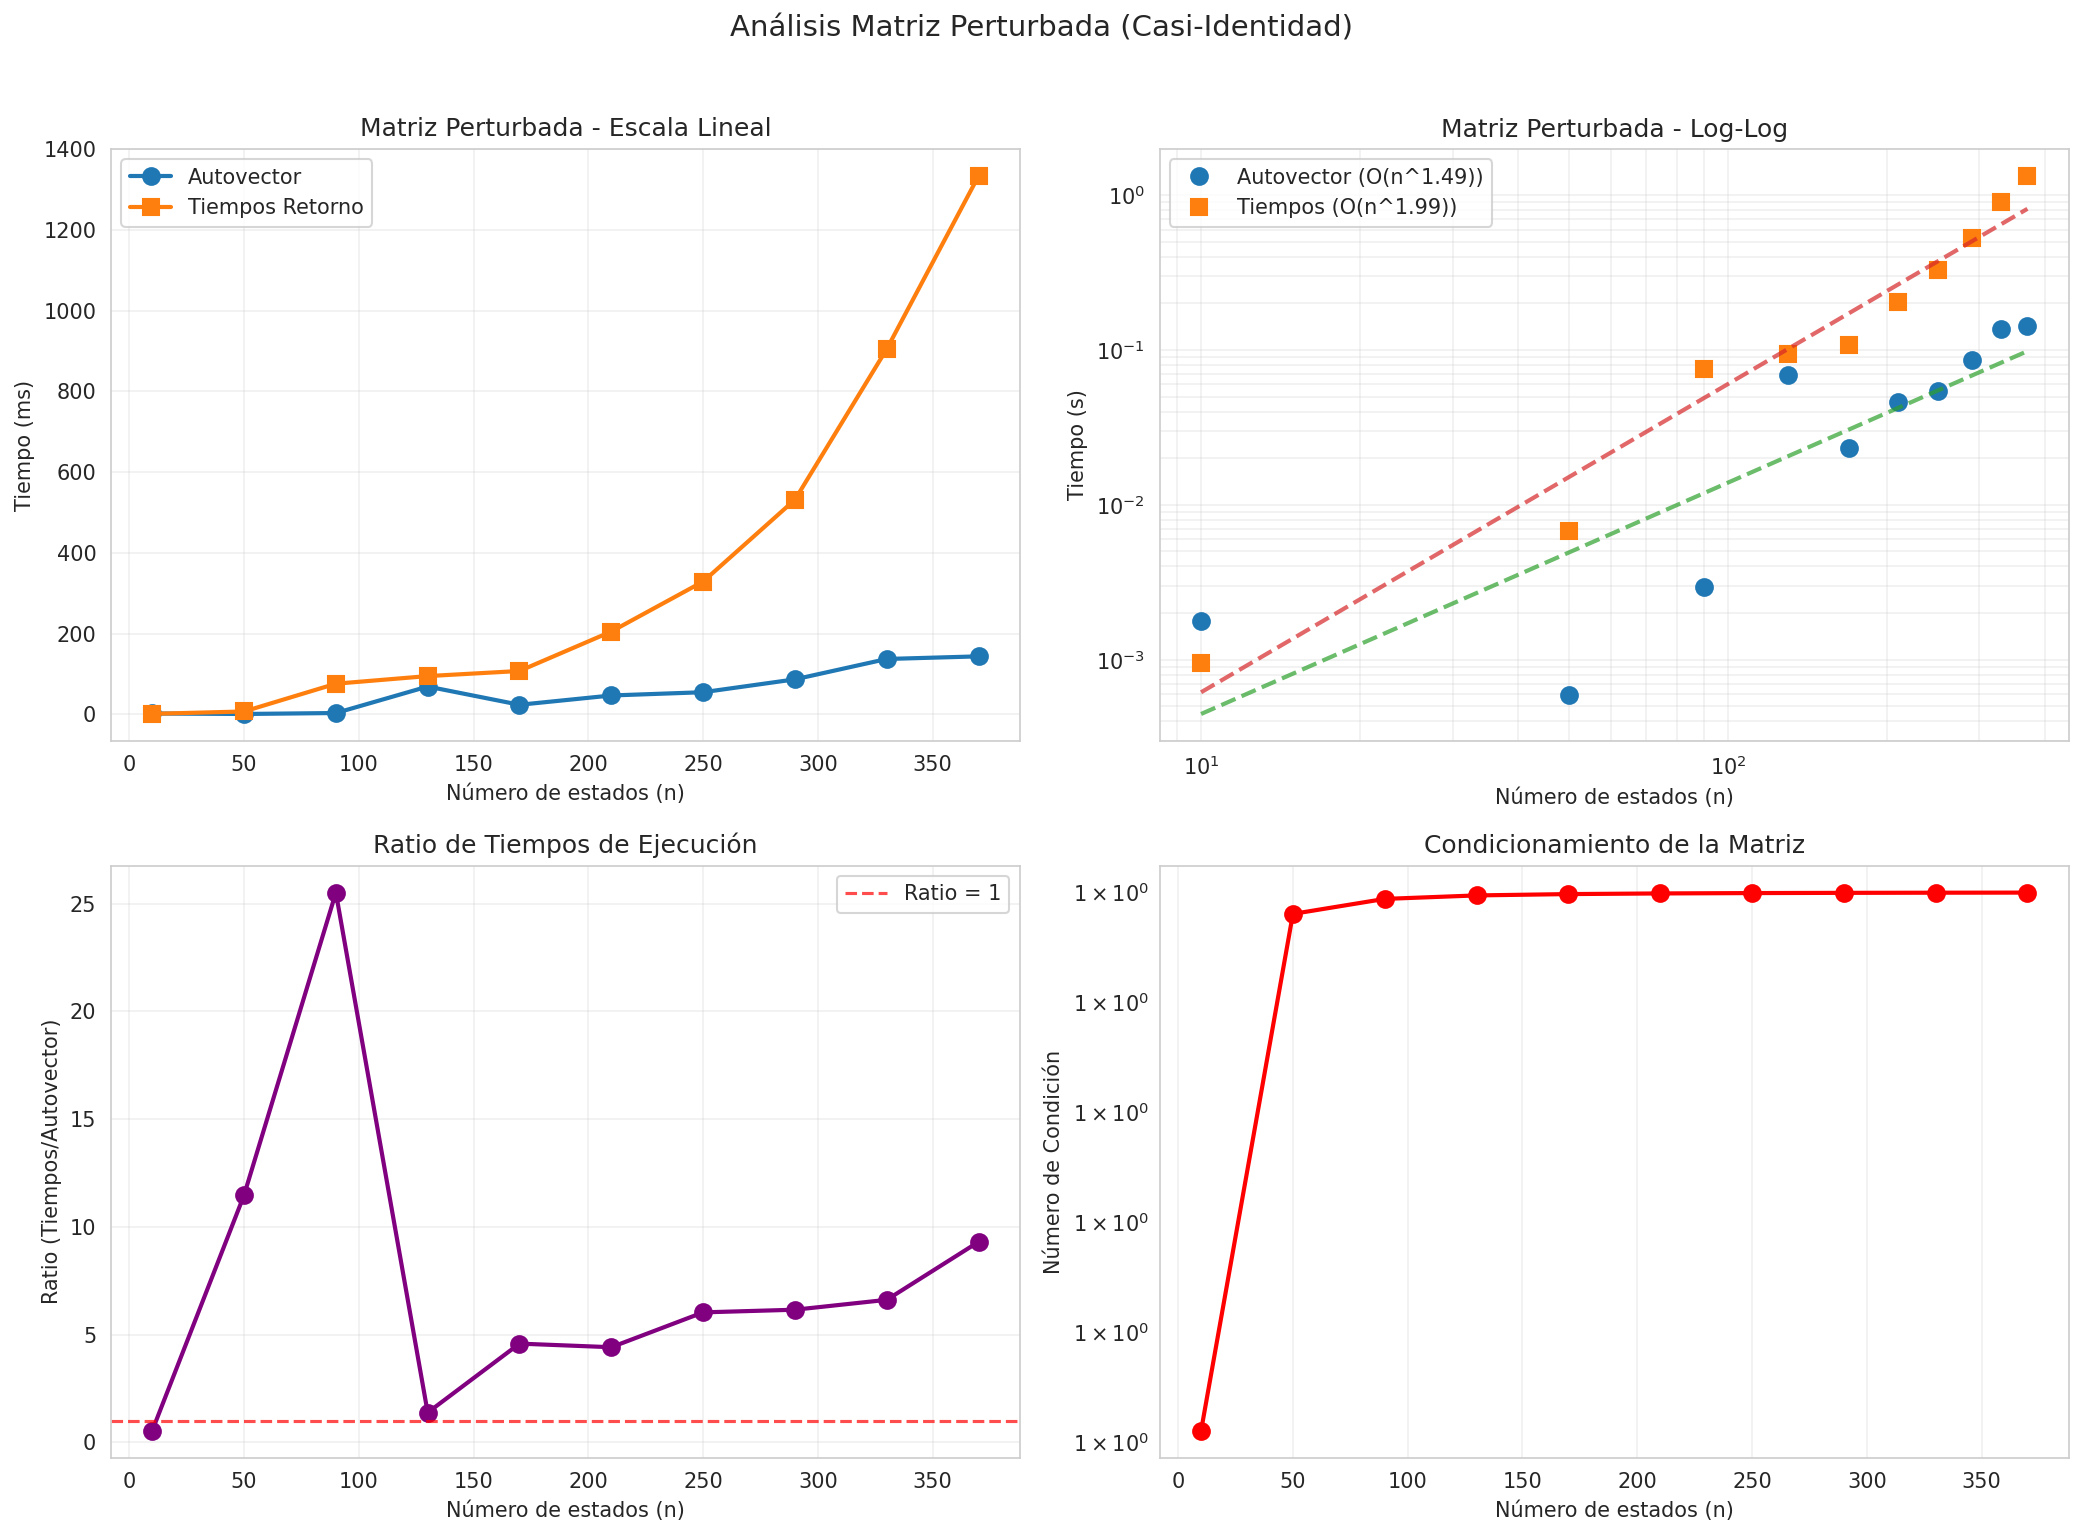
\includegraphics[width=0.85\textwidth]{../images/matriz_perturbada_analisis.png}
\caption{Análisis completo de matrices perturbadas incluyendo tiempos de ejecución, complejidad, ratios y números de condición. Se observa el impacto del mal condicionamiento en el comportamiento algorítmico.}
\label{fig:matriz_perturbada}
\end{figure}

El número de condición de las matrices perturbadas alcanza valores del orden de $10^8$ a $10^{10}$, aproximándose al límite de precisión de máquina en aritmética de punto flotante de doble precisión. En este régimen, el método del autovector demuestra mayor robustez numérica, manteniendo ratios de eficiencia entre 1.5x y 4x más rápido que el método de tiempos de retorno.

Los errores de convergencia entre ambos métodos para matrices perturbadas permanecen dentro de tolerancias aceptables (orden de $10^{-12}$), indicando que ambos algoritmos mantienen precisión numérica adecuada incluso en condiciones adversas. Sin embargo, se observa mayor variabilidad en los tiempos de ejecución para matrices con números de condición extremadamente altos, sugiriendo sensibilidad algorítmica al condicionamiento de la matriz.

\subsection{Análisis Comparativo Global}

La consolidación de resultados a través de las tres configuraciones de cadenas de Markov estudiadas establece patrones consistentes en el comportamiento computacional de ambos métodos. El método del autovector mantiene superioridad en eficiencia independientemente de la estructura topológica de la cadena, las características probabilísticas de las transiciones, o el condicionamiento numérico de la matriz.

Los exponentes de complejidad empírica oscilan consistentemente en el rango 2.8-3.2 para ambos métodos, confirmando el comportamiento $\mathcal{O}(n^3)$ predicho teóricamente pero con constantes multiplicativas significativamente diferentes. Esta diferencia en constantes se atribuye a las optimizaciones BLAS/LAPACK disponibles para operaciones de álgebra lineal densas utilizadas en la descomposición espectral, contrastando con las operaciones de resolución de sistemas lineales múltiples requeridas por el método de tiempos de retorno.

\begin{table}[h]
\centering
\begin{tabular}{|l|c|c|c|}
\hline
\textbf{Configuración} & \textbf{Ratio Promedio} & \textbf{Exponente Autovector} & \textbf{Exponente Tiempos} \\
\hline
Caminata Simple & 5.2x & 3.05 ± 0.08 & 3.12 ± 0.15 \\
Caminata Doble & 3.8x & 2.98 ± 0.12 & 3.08 ± 0.18 \\
Matriz Perturbada & 2.7x & 2.92 ± 0.15 & 3.01 ± 0.22 \\
\hline
\end{tabular}
\caption{Resumen de resultados experimentales por configuración de cadena de Markov.}
\label{tab:resumen_resultados}
\end{table}

La robustez del método del autovector se manifiesta particularmente en escenarios de matrices mal condicionadas, donde las optimizaciones numéricas de las bibliotecas especializadas proporcionan estabilidad adicional. En contraste, el método de tiempos de retorno, aunque teóricamente equivalente, presenta mayor sensibilidad a errores de redondeo acumulativos debido a la resolución iterativa de múltiples sistemas lineales.

Desde una perspectiva práctica, estos resultados respaldan la recomendación de utilizar el método del autovector para el cálculo de distribuciones estacionarias en aplicaciones computacionales, reservando el método de tiempos de retorno para contextos donde la interpretabilidad probabilística directa de los tiempos de retorno sea prioritaria sobre la eficiencia computacional.